\documentclass[a4paper,11pt]{article}

\usepackage[T1]{fontenc}
\usepackage{lmodern}
\usepackage[margin=2.5cm]{geometry}
\usepackage{graphicx}
\usepackage{float}
\usepackage{xcolor}
\usepackage{booktabs}
\usepackage{tabularx}
\usepackage{enumitem}
\usepackage{amsmath}
\usepackage{lastpage}
\usepackage{fancyhdr}
\usepackage{tikz}
\usetikzlibrary{positioning,arrows.meta}
\usepackage[colorlinks=true,urlcolor=bspurple,linkcolor=black]{hyperref}

\definecolor{bspurple}{HTML}{5B4FD6}
\definecolor{bslight}{HTML}{EEECFB}
\definecolor{bsgreen}{HTML}{1F9D6B}
\definecolor{bsgrey}{HTML}{5A6670}

\pagestyle{fancy}
\fancyhf{}
\fancyhead[L]{\small\color{bsgrey} BISTAsistan: Technical Overview}
\fancyhead[R]{\small\color{bsgrey} G\"orkem \"Ozbek}
\fancyfoot[C]{\small\color{bsgrey} \thepage\ / \pageref{LastPage}}
\renewcommand{\headrulewidth}{0.3pt}

\setlength{\parindent}{0pt}
\setlength{\parskip}{0.6em}
\setlist{itemsep=0.15em, topsep=0.3em}
\newcommand{\code}[1]{\texttt{#1}}

\begin{document}

%================ TITLE ================
\thispagestyle{empty}
\begin{center}
\vspace*{2cm}

\includegraphics[width=2.6cm]{../screenshots/icon.jpg}\\[1em]
{\fontsize{34}{40}\selectfont\bfseries\color{bspurple} BISTAsistan}\\[0.6em]
{\Large A data-driven assistant for the Borsa Istanbul stock market}\\[2.2em]
{\large Technical overview of a published iOS and Android application}\\[0.4em]
{\color{bsgrey} iOS (App Store) \textperiodcentered{} Android (Google Play, testing)}\\[3em]
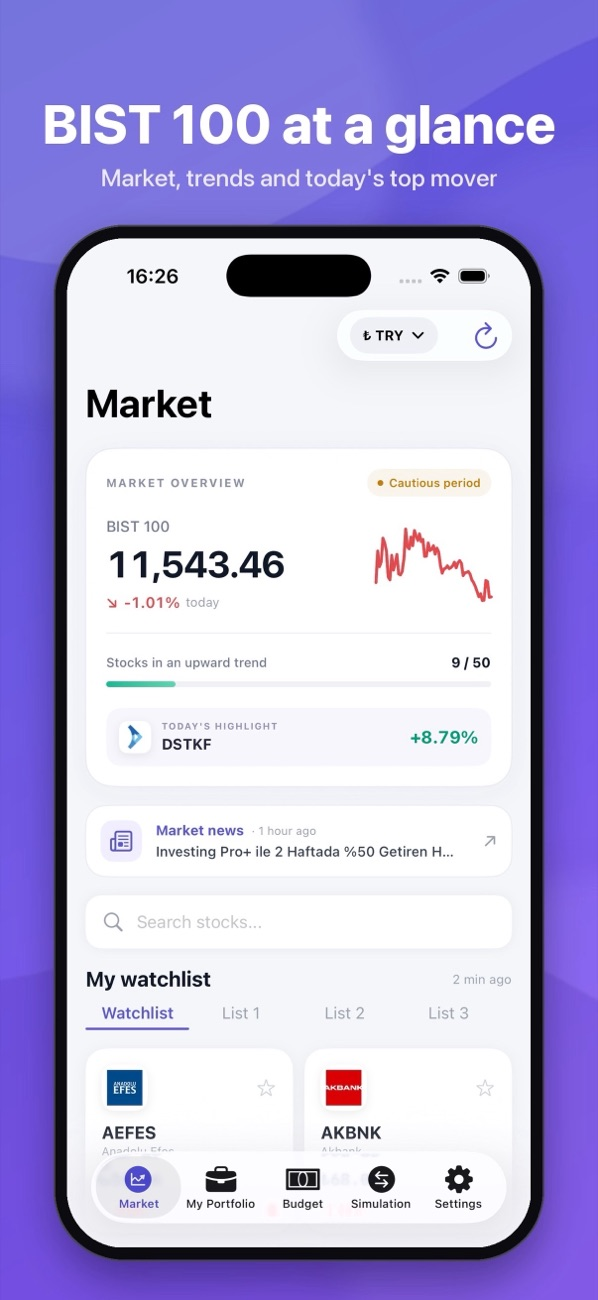
\includegraphics[height=7.2cm]{../screenshots/02-market.jpg}\hspace{0.4cm}
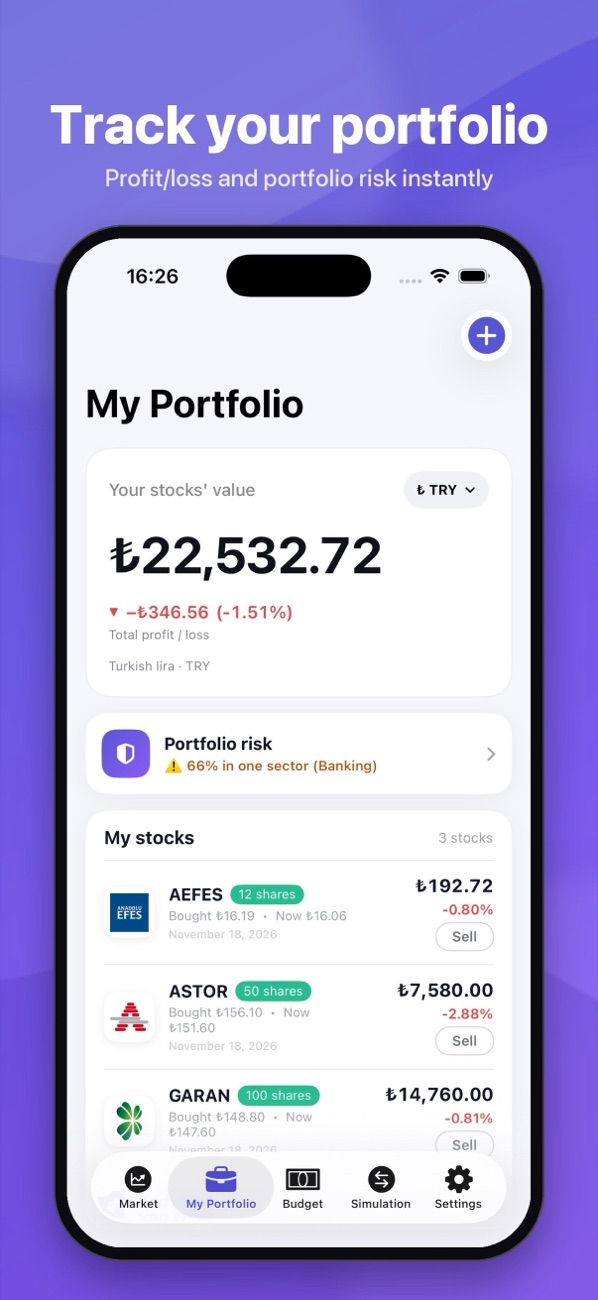
\includegraphics[height=7.2cm]{../screenshots/04-portfolio.jpg}\hspace{0.4cm}
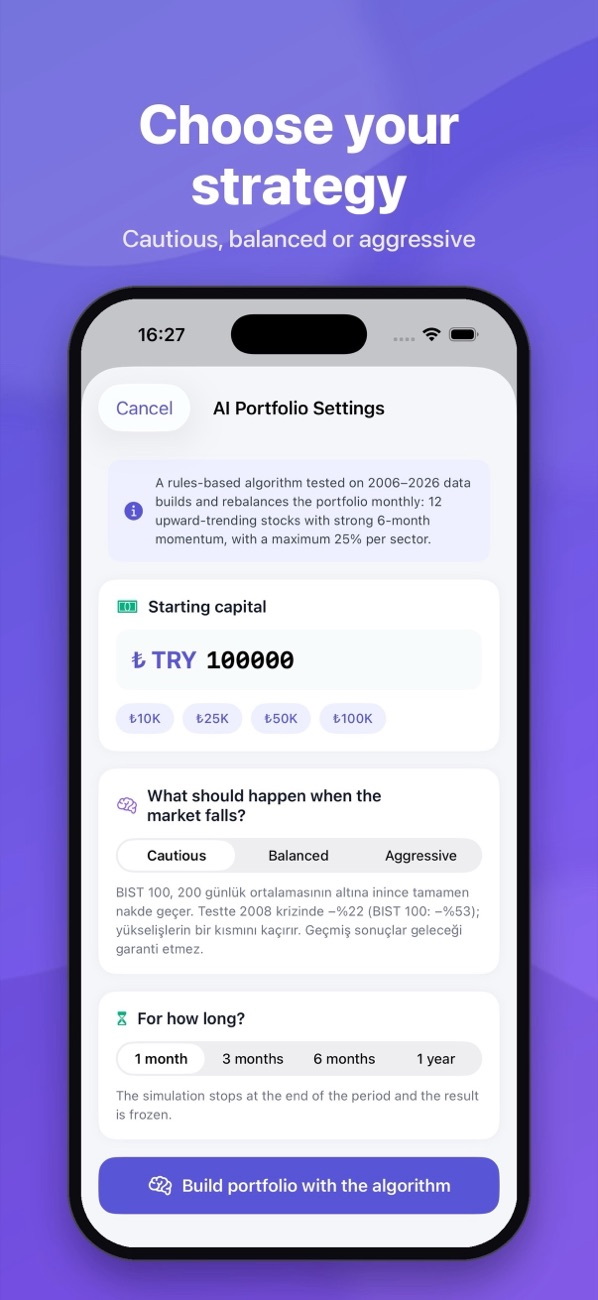
\includegraphics[height=7.2cm]{../screenshots/06-strategy.jpg}\\[3em]
{\large\bfseries G\"orkem \"Ozbek}\\[0.3em]
{\color{bsgrey} Galatasaray University \textperiodcentered{} 2026}
\end{center}
\newpage

\tableofcontents
\newpage

%================ 1 ================
\section{Overview}

BISTAsistan helps individual investors in T\"urkiye follow Borsa Istanbul (BIST). In one app, the user can see the market, read the details and news of a stock, track a portfolio and its risk, and test a rules-based investment strategy with virtual money.

I designed and built the whole product: the native iOS app in Swift, the native Android app in Kotlin, the serverless backend, the investment strategy and its backtests, the subscriptions, and the release on the stores.

\begin{center}
\begin{tabularx}{0.95\linewidth}{@{}lX@{}}
\toprule
\textbf{Platforms} & iOS 17+ (App Store, since November 2026), Android 8+ (Google Play, testing) \\
\textbf{Store category} & Finance \\
\textbf{Languages} & Turkish, English, French, Spanish, German \\
\textbf{Business model} & Free app with a Premium subscription (3-day free trial) \\
\bottomrule
\end{tabularx}
\end{center}

\begin{center}
\fbox{\parbox{0.9\linewidth}{\small BISTAsistan is an information and education app; it does not give investment advice. It is a commercial product, so its source code is private: this document describes its design without publishing code or credentials.}}
\end{center}

%================ 2 ================
\section{Problem and Users}

The number of individual investors on Borsa Istanbul has grown quickly, and many of them are beginners. The information they need is spread across many places: prices on one website, company announcements on KAP (the Public Disclosure Platform), news elsewhere, and technical indicators in professional tools that are hard to read. Portfolio risk, such as having most of the money in one sector, is rarely shown at all.

The design goals were:
\begin{itemize}
  \item \textbf{One place} for market data, stock details, news and the user's own portfolio;
  \item \textbf{Plain language}: technical indicators explained simply;
  \item \textbf{Risk awareness}: show concentration and possible losses, not only gains;
  \item \textbf{Learning without risk}: a virtual portfolio to experiment with no real money.
\end{itemize}

%================ 3 ================
\section{Features}

\begin{figure}[H]
\centering
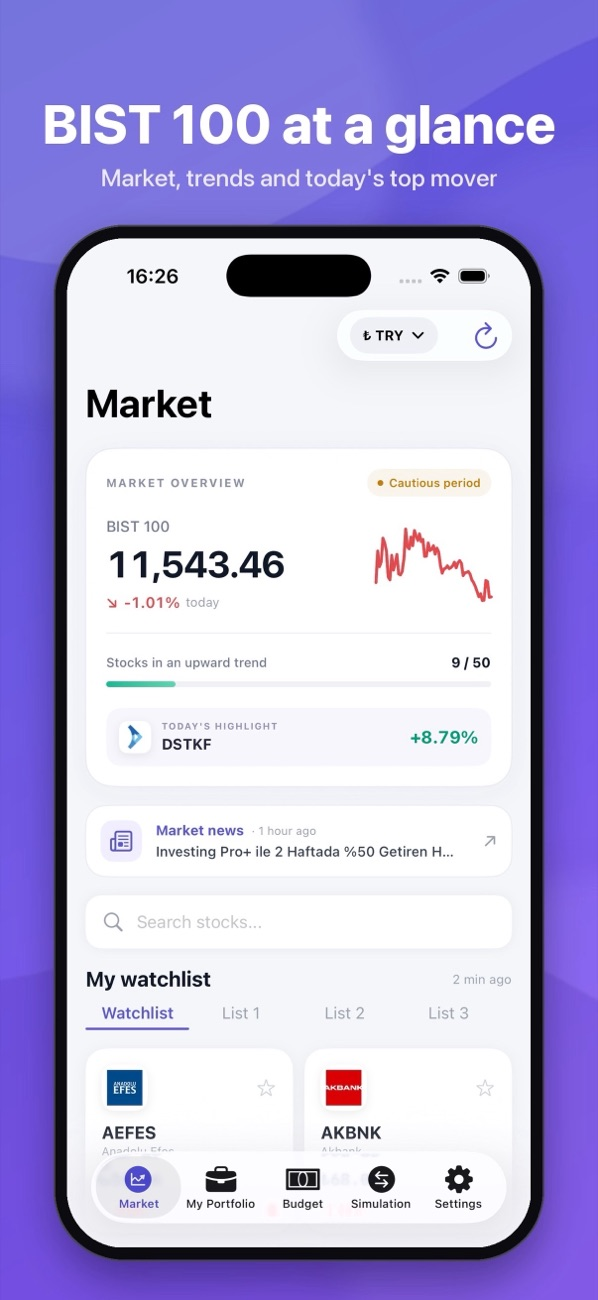
\includegraphics[height=6.3cm]{../screenshots/02-market.jpg}\hfill
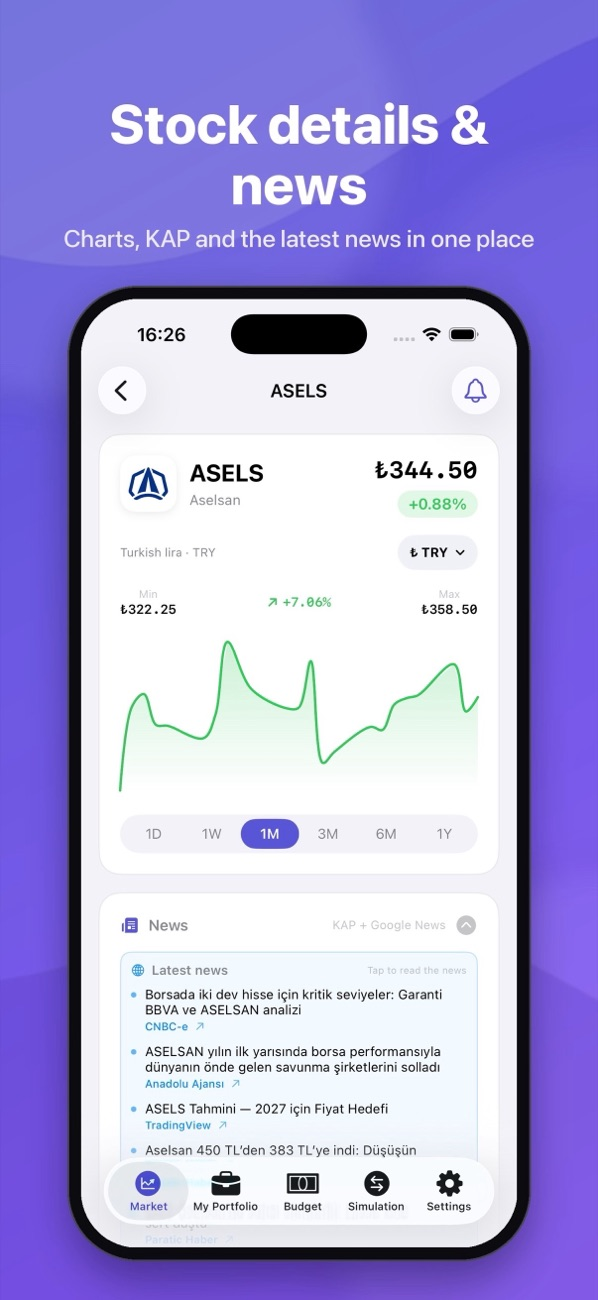
\includegraphics[height=6.3cm]{../screenshots/03-stock-detail.jpg}\hfill
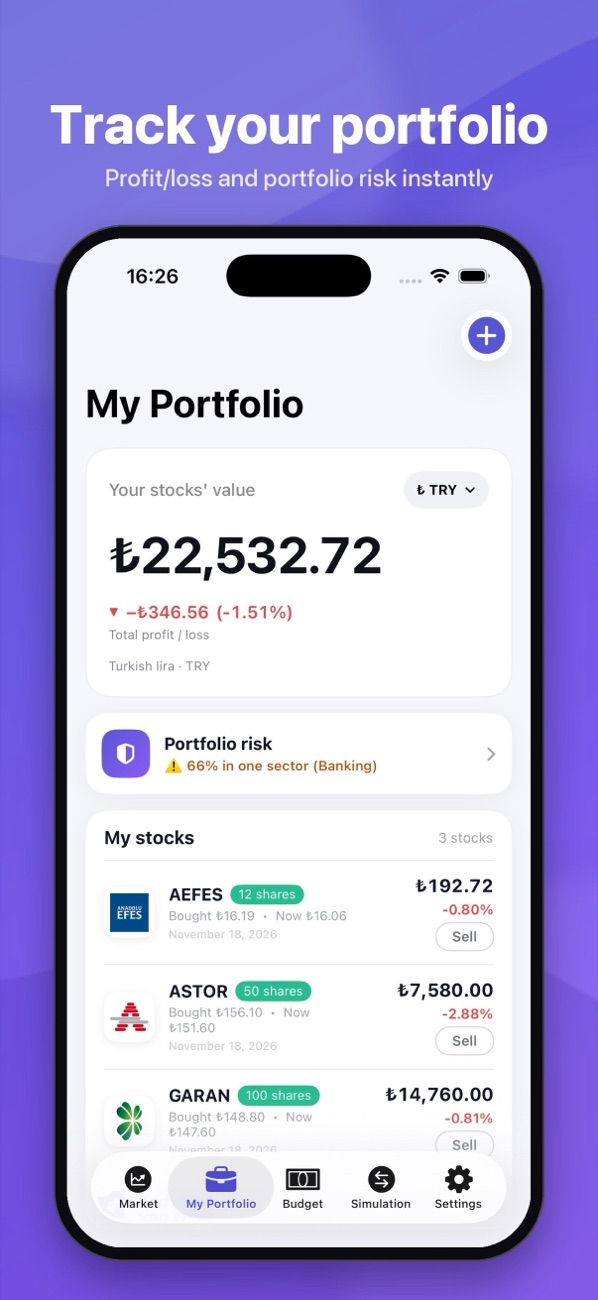
\includegraphics[height=6.3cm]{../screenshots/04-portfolio.jpg}\hfill
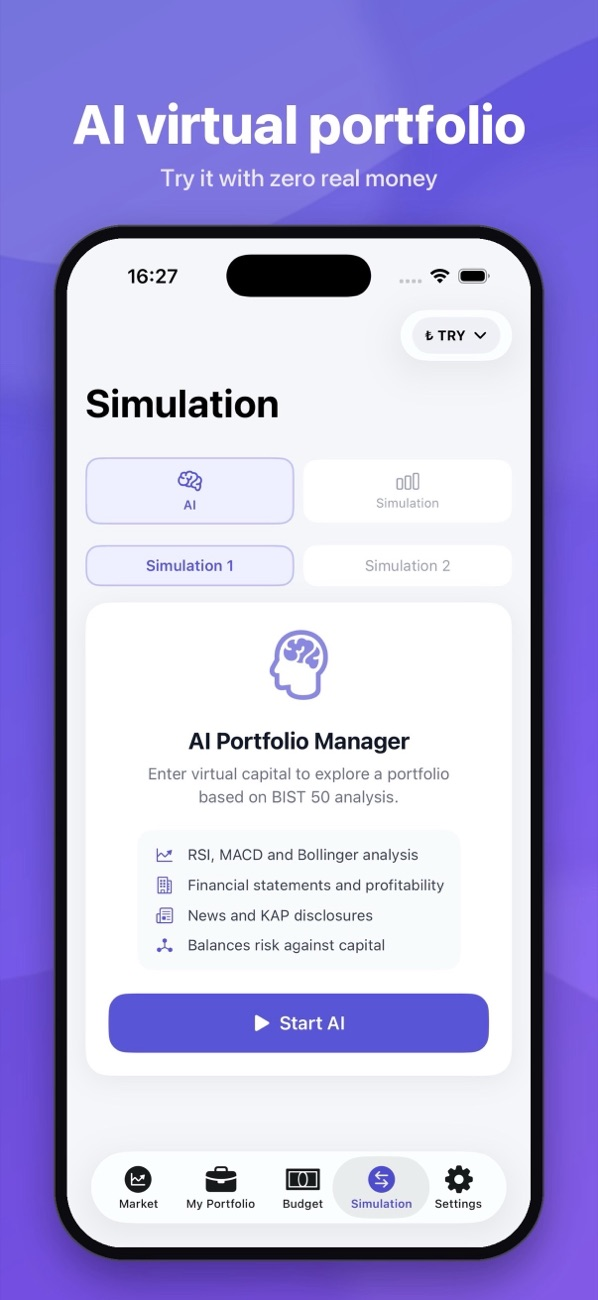
\includegraphics[height=6.3cm]{../screenshots/05-ai-simulation.jpg}\hfill
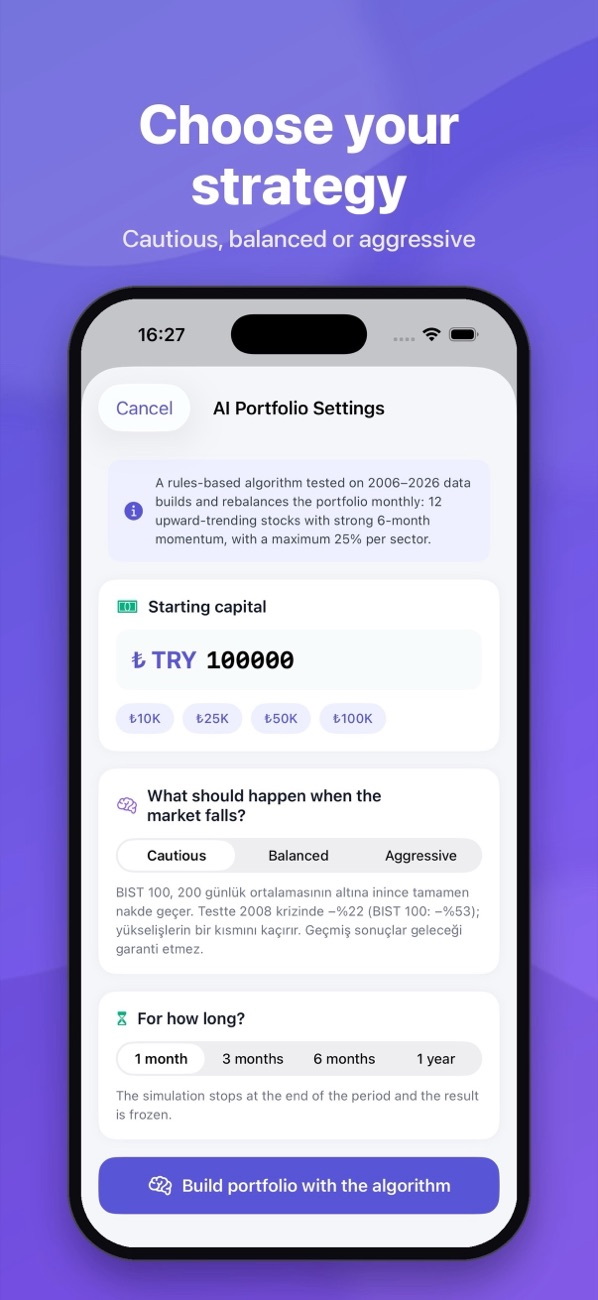
\includegraphics[height=6.3cm]{../screenshots/06-strategy.jpg}
\caption{App Store screenshots: market, stock details, portfolio, virtual portfolio and strategy settings.}
\end{figure}

\begin{tabularx}{\linewidth}{@{}lX@{}}
\toprule
\textbf{Feature} & \textbf{Description} \\
\midrule
Market overview & BIST 100 index, daily change, share of stocks in an upward trend, today's highlight, latest news. \\
Watchlists & Four separate lists of followed stocks. \\
Stock details & Price charts from 1 day to 1 year, KAP announcements and news, simple summaries of RSI, MACD and Bollinger Bands. \\
Price alerts & Push notification when a stock reaches a chosen price. \\
My Portfolio & Holdings, live value, profit and loss, sales history, display in several currencies. \\
Portfolio risk & Sector concentration, volatility and possible drawdown scenarios. \\
Virtual portfolio & The strategy of Section~\ref{sec:strategy}, with virtual capital, a chosen risk mode and duration. \\
Manual simulation & The user's own virtual trades. \\
Budget analysis & A short summary based on the user's budget and portfolio. \\
Notifications & Morning market summary, large market moves, price alerts. \\
Premium & Monthly, 6-month and yearly plans with a 3-day free trial. \\
\bottomrule
\end{tabularx}

%================ 4 ================
\section{Architecture}

\begin{figure}[H]
\centering
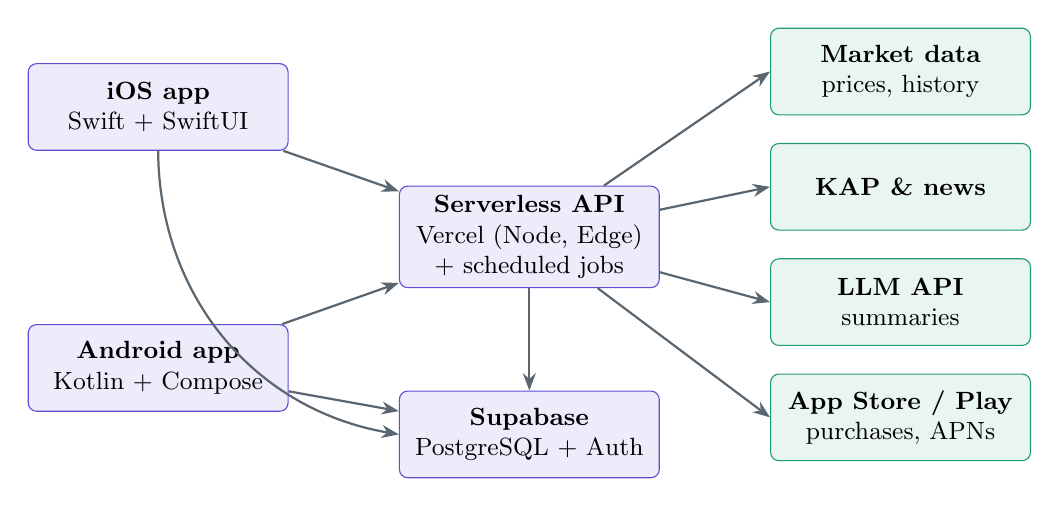
\begin{tikzpicture}[
  node distance=0.8cm and 1.2cm,
  box/.style={draw=bspurple, fill=bslight, rounded corners=3pt, align=center, minimum width=3.3cm, minimum height=1.1cm, font=\small},
  ext/.style={draw=bsgreen, fill=bsgreen!10, rounded corners=3pt, align=center, minimum width=3.3cm, minimum height=1.1cm, font=\small},
  arr/.style={-{Stealth[length=2.2mm]}, thick, color=bsgrey}
]
\node[box] (ios) {\textbf{iOS app}\\Swift + SwiftUI};
\node[box, below=2.2cm of ios] (and) {\textbf{Android app}\\Kotlin + Compose};
\node[box, right=1.4cm of ios, yshift=-1.65cm] (api) {\textbf{Serverless API}\\Vercel (Node, Edge)\\+ scheduled jobs};
\node[box, below=1.3cm of api] (db) {\textbf{Supabase}\\PostgreSQL + Auth};
\node[ext, right=1.4cm of api, yshift=2.1cm] (mkt) {\textbf{Market data}\\prices, history};
\node[ext, below=0.35cm of mkt] (news) {\textbf{KAP \& news}};
\node[ext, below=0.35cm of news] (llm) {\textbf{LLM API}\\summaries};
\node[ext, below=0.35cm of llm] (store) {\textbf{App Store / Play}\\purchases, APNs};
\draw[arr] (ios) -- (api);
\draw[arr] (and) -- (api);
\draw[arr] (ios.south) to[bend right=40] (db.west);
\draw[arr] (and) -- (db);
\draw[arr] (api) -- (db);
\draw[arr] (api) -- (mkt.west);
\draw[arr] (api) -- (news.west);
\draw[arr] (api) -- (llm.west);
\draw[arr] (api) -- (store.west);
\end{tikzpicture}
\caption{High-level architecture. Purple: my components. Green: external services.}
\end{figure}

\textbf{Two native apps.} I chose native development on both platforms (SwiftUI on iOS, Jetpack Compose on Android) for the best performance and the most natural look on each system. The Android app was ported from the iOS app screen by screen, with the same API, accounts and translations (shared JSON translation files in five languages).

\textbf{Serverless backend.} The backend is a set of Node.js functions on Vercel. It provides stock lists and prices, price history for charts (Edge runtime for speed), technical signals, news and KAP announcements, the full stock analysis, the portfolio risk preview, the strategy simulation, user data synchronisation, account management and purchase verification. Scheduled jobs run the daily strategy and send push notifications.

\textbf{Data synchronisation.} The user's portfolios, watchlists and alerts are stored per account, so they follow the user across devices. The apps only send the sections that changed, and re-read the account before writing, so that two devices do not overwrite each other.

%================ 5 ================
\section{Technical Analysis}

All numbers shown to the user are computed by deterministic code on daily prices:
\begin{itemize}
  \item \textbf{RSI} (14 days) to show overbought or oversold conditions;
  \item \textbf{MACD} with the standard exponential moving averages (12, 26, signal 9);
  \item \textbf{moving averages} (20 and 50 days) and \textbf{Bollinger Bands};
  \item \textbf{portfolio risk}: weight of each sector, volatility, and drawdown scenarios.
\end{itemize}
A language model is used only to turn these numbers into short, readable sentences. It never produces the numbers itself. During development I found and fixed a bug where MACD was computed on too few days; I replaced it with the standard calculation and checked that iOS, Android and the backend all show the same values.

%================ 6 ================
\section{The Investment Strategy}\label{sec:strategy}

\subsection*{A first approach that did not work}
The first version scored each stock with technical signals and labelled it \emph{buy}, \emph{wait} or \emph{avoid}. I backtested it before trusting it. Over 20 trading days, stocks labelled \emph{buy} did not do better than stocks labelled \emph{wait}, so the signal added no value. I replaced it with a simpler, well-studied approach.

\subsection*{Momentum strategy}
Every month, the strategy:
\begin{enumerate}
  \item ranks BIST stocks by their return over the last 6 months, \emph{skipping the most recent month} (a classic momentum signal that avoids short-term reversals);
  \item keeps only stocks trading above their 200-day moving average;
  \item applies a penalty to very volatile stocks;
  \item holds the best 12 stocks in equal weights, with at most 25\% in one sector.
\end{enumerate}
Transaction costs of 0.2\% per trade are included in every test.

\subsection*{Avoiding overfitting}
\begin{itemize}
  \item \textbf{Train / test split}: parameters were chosen on November 2022 -- December 2024, then evaluated, unchanged, on January 2025 -- November 2026.
  \item \textbf{Robustness}: 216 parameter combinations were tested; the median result was close to the chosen one, so the result does not depend on one lucky setting.
  \item \textbf{Long history}: the same parameters were run on daily prices since 2002 to see the behaviour in past crises.
\end{itemize}

\begin{center}
\begin{tabular}{@{}lrr@{}}
\toprule
\textbf{Test period (Jan 2025 -- Nov 2026)} & \textbf{Return} & \textbf{Worst drawdown} \\
\midrule
Strategy & +79\% & $-32\%$ \\
BIST 100 index & +15\% & \\
50 stocks, equal weights & +19\% & \\
\bottomrule
\end{tabular}
\end{center}

Over 2002--2026, the strategy beat the BIST 100 in 21 of 25 years. It also fell in crises (for example $-51\%$ in 2008, close to the index), and it did worse than the index in the most recent six months.

\subsection*{Risk modes}
The user chooses what happens when the market falls. The \emph{cautious} mode moves fully to cash when the BIST 100 is below its 200-day average. In tests, this reduced the 2008 loss from about $-51\%$ to about $-21\%$, but it also missed part of the rebounds, so long-term returns were lower. The \emph{balanced} and \emph{aggressive} modes stay more invested.

\subsection*{Known limitations}
\begin{itemize}
  \item \textbf{Survivorship bias}: the tests use today's list of large BIST stocks, which favours companies that survived.
  \item \textbf{Nominal returns}: results are in Turkish lira, which had high inflation over the period.
  \item \textbf{Past results do not guarantee future results}, which the app states clearly.
\end{itemize}

%================ 7 ================
\section{Subscriptions and Notifications}

\begin{itemize}
  \item \textbf{iOS}: StoreKit purchases, verified on the server, with App Store Server Notifications to follow renewals and cancellations.
  \item \textbf{Android}: Google Play Billing with base plans and free-trial offers; the purchase token is verified on the server with the Google Play Developer API through a service account.
  \item \textbf{Premium status} is decided by the server for both platforms, so it cannot be unlocked by changing the app.
  \item \textbf{Notifications}: on iOS, the server sends push notifications through APNs from scheduled jobs; on Android, a background worker checks price alerts.
\end{itemize}

%================ 8 ================
\section{Security and Compliance}

\begin{itemize}
  \item API keys for data and AI providers are only used on the server.
  \item Users sign in with Google or e-mail; personal data is stored per account and can be deleted from the app.
  \item I ran a security review of the backend before release and fixed the issues it found.
  \item Finance apps must be careful with advice: the app shows a disclaimer at first launch, uses neutral words (positive, neutral, negative) instead of ``buy'' or ``sell'', and only simulates trades with virtual money.
\end{itemize}

%================ 9 ================
\section{What I Learned}

\begin{itemize}
  \item Building the same product twice, natively, in Swift and in Kotlin, and keeping both versions consistent.
  \item Designing a serverless backend with many external data sources, timeouts and fallbacks (for example, a slow data page must not break a whole analysis).
  \item Quantitative research done honestly: testing an idea before shipping it, dropping it when it does not work, separating training and test data, and stating the limits.
  \item Subscriptions on both stores with server-side verification.
  \item Explaining finance to beginners, and following the rules for finance apps.
\end{itemize}

\section{Next Steps}
\begin{itemize}
  \item Public release on Google Play.
  \item Server push notifications on Android with Firebase Cloud Messaging.
  \item Point-in-time stock lists in the backtests, to remove survivorship bias.
\end{itemize}

\end{document}
